
%*****************************************
\chapter{Theme}\label{ch:second}
%*****************************************

The purpose of this chapter is to fill the gap of knowledge on \textbf{smartphone authentication}, by contextualizing its importance and by illustrating why its improvement is crucial and necessary. Next, we will introduce the research field of \textbf{Usable Security} by explaining its aim and portray the steps that researchers are taking to increase usability in security mechanisms, in general. Last but not least, we will present the recent work and approaches made in the field of improving usability in smartphone authentication.   

\section{Context}

\subsection{Importance of Smartphone Authentication} \label{2.1.1}

Nowadays, smartphones are approved to be one of the main essentials in people's day to day lives. Besides serving as a medium for essential communication, mobile phones have evolved remarkably, offering advanced features and functions which were formally known to only be possible on a personal computer \cite{Alsaleh}. Besides storing and granting access to private photos, videos, emails, and social media, smartphones enable their users to do money transfers, online shopping and even track their health through the tips of their fingers \cite{Egelman:2014:YRL:2660267.2660273,Albayram:2017:BUL:3235924.3235929,Schloeglhofer}. \\

Being the powerful and capable devices that they are, it is said that smartphones have the potential to replace the need for a personal desktop \cite{Alsaleh}. Hence, they should be capable of protecting their users' sensitive and private data confidentially and securely. The fact that users carry their mobile phones with them wherever they go causes a threat that the devices might get lost or even stolen \cite{Egelman:2014:YRL:2660267.2660273}. An American software company, named \textbf{Symantec}\footnote{https://www.symantec.com/de/de - last accessed: 2019/11/04}, conducted an experiment, where they purposely "lost" fifty unprotected smartphones in five destinations. They did so, to observe how the finders of the devices would behave and how they would treat the data stored on the devices. Surprisingly, they found that the data was accessed on 96\% of the smartphones and that only half of the finders offered to return the devices \cite{symantec}.  This experiment portrays a security risk that is likely to affect any smartphone user.  It is safe to assume that a smaller amount of the data would have been compromised, had the phones been protected by a security mechanism. Therefore, securing smartphones with an authentication mechanism is vital for users' data security and privacy.\\

The purpose of an \textbf{authentication mechanisms} is to allow a person access to a particular medium, only after verifying and approving that they indeed are who they claim to be. There are many ways in which this could take place. In general, the mechanism asks the person, requesting access, to enter a secret which only the owner of the medium should know. It serves as a countermeasure to the exploitation of personal and confidential information. There are many types of authentication mechanisms, and these can be categorised as follows \cite{gorman}: 
\begin{itemize}
    \item \textbf{Biometric} - describes "what You are" e.g., fingerprint scanner and facial recognition.
    \item \textbf{Knowledge-Based} - describes "what You know" e.g., pattern, password, pin.
    \item \textbf{Token-Based} - describes "what You have" e.g., cryptographic key or chip.
\end{itemize}


When speaking of authentication in smartphones, there are a couple of well-known mechanisms that come to mind. These can also be categorized as follows \cite{ediss20251,gorman} : 
\begin{itemize}
    \item \textbf{Alphanumeric} e.g., password and pin
    \item \textbf{Gesture-Based} e.g., Android Unlock Pattern
    \item \textbf{ID-Based} e.g., fingerprint scanner and facial recognition 
\end{itemize}

To this day, researchers have been working on improving authentication in smartphones and developing new concepts and designs for them. One might wonder why this is necessary when there is a hand full of methods already available. Are the current mechanisms not sufficient or secure enough? The answer to this question is twofold:\\

On the one hand, specific authentication mechanisms lack in security and are vulnerable towards certain attacks \cite{Schloeglhofer}. For instance, Android Unlock Pattern is known to be vulnerable towards so-called \textbf{smudge attacks}. These are attacks that occur when a victim has previously drawn their secret pattern, leaving an oily trace of their finger on the touch screen. These smudge marks help the attacker to guess the secret pattern, bypass the security measure, and gain access to the device \cite{ediss20251}. Another popular attack, which occurs primarily "in the wild" are \textbf{shoulder surfing attacks}. These happen when the victim attempts to authenticate themself in public and uncontrolled surroundings. If the attacker is situated in a near distance, behind or beside the victim, they can observe the input of the secret and memorize it for later use \cite{ediss20251}. Authentication mechanisms (e.g. pin, password, and Android Unlock Pattern) are prone to such threats, especially when the alphanumeric or pattern secrets are short and simple enough to memorize easily. There have been many research contributions that propose improvements of existing mechanisms as well as the development of new ones to counteract these security threats. Zezschwitz et al. \cite{vonZezschwitz:2015:SFS:2702123.2702212} developed an interesting authentication concept called \textbf{SwiPIN}, intended to protect pin authentication from shoulder surfing attacks. Another proposal, \textbf{Tinylock}, made by Kwon et al. \cite{kwon}, acts against both smudge and shoulder surfing attacks.\\


On the other hand, certain authentication mechanisms still lack in user-friendliness and are therefore not as usable as their developers intend for them to be \cite{Schloeglhofer}. As a result, research has shown that many users consciously choose not to use an authentication mechanism on their smartphones \cite{ediss20251, Albayram:2017:BUL:3235924.3235929, Egelman:2014:YRL:2660267.2660273}. Studies have indicated that one of the main reasons for such behavior is that users perceive screen locks as an inconvenience \cite{Albayram:2017:BUL:3235924.3235929, ediss20251, harbach}. Another reason was found to be a lack of knowledge about smartphone security \cite{Albayram:2017:BUL:3235924.3235929, Adams:1999:UE:322796.322806}. Researchers discovered that some users decide not to install a screen lock, because they underestimate the risk that comes with not having one and because they do not comprehend to which extent their data is at stake \cite{Egelman:2014:YRL:2660267.2660273}. Through finding out this information, investigations were made on how to create authentication mechanisms that aren't just secure, but also usable. On that note, studies have been made on examining authentication from the user's perspective and finding out ways to create concepts that satisfy both sides: \textbf{usability} and \textbf{security}.  


\subsection{Improving Usability in Smartphone Authentication}

As mentioned earlier, security, alone, is not sufficient enough to guarantee the true success of an authentication mechanism. A lack of usability in security mechanisms defeats their purpose, no matter how secure they are in theory. \textbf{Usable security} is a growing, and widely popular research field whose aim is to create a balance between \textbf{usability} and \textbf{security} in security systems and mechanisms \cite{Realpe-Munoz, anonymous}. In order to better understand their ambitions, we will first give an understanding of what usability is. \\

\textbf{Usability} generally describes the degree to which a user can accomplish a certain task with "effectiveness, efficiency, and satisfaction" when utilizing a certain product.\footnote{https://www.interaction-design.org/literature/topics/usability - Last accessed: 2019/11/10} While this definition applies to all designed and developed products imaginable, it certainly also applies to security mechanisms. The goal of usable security experts is to construct the design process for a security measure similar to the design for any product intended for human use. In other words, security designers should implement a user-centered approach when designing security mechanisms in order to involve certain human factor principles, crucial to their success \cite{Adams:1999:UE:322796.322806, sasse}. Interestingly, the importance of usability was initially established in 1975 in a research article titled \textit{"The Protection of Information in Computer Systems"}. To our knowledge, the relevance of user-centered design was first introduced nearly two decades ago in an article called \textit{"Users are not the enemy"} \cite{Adams:1999:UE:322796.322806}. \\

Despite previous discoveries, usability of authentication mechanisms remains a conundrum waiting to be solved. While users find it hard to comply with required security guidelines and therefore behave insecurely \cite{Adams:1999:UE:322796.322806, sasse}, security experts perceive users as \textit{"the weakest link in the chain of system security"} \cite{sasse} and find that they are \textit{"a security risk that needs to be controlled and managed"}  \cite{Adams:1999:UE:322796.322806}. Hackers have learned how to benefit from this situation by using social engineering methods to obtain individuals' authentication secrets \cite{Adams:1999:UE:322796.322806, sasse}. They notice the flaws in current security systems and can foresee how users will behave. Users, however, are not to blame for this issue entirely. The reason why hackers are able to attain unauthorized access to systems so easily is that they are more attentive to users' perception of security than security designers are \cite{Adams:1999:UE:322796.322806}. By nature, humans are prone to try and find shortcuts and time-saving methods when it comes to challenging tasks \cite{sasse}. This behavior applies when using security mechanisms which demand actions that are either impossible or unnatural to follow \cite{sasse}. For instance, when using a password-protected system, requirements are to use an alphanumerical secret that is at least eight characters long, consists of lower and upper case letters as well as special characters \cite{payne, sasse}. \\

Furthermore, passwords are required to be changed regularly \cite{adams2,gorman}. These regulations might be easy to comply with when the user only has one password to memorize. However, nowadays, users have to manage a multitude of passwords, which makes following the guidelines more tiresome and difficult. To that end, users are bound to seek a solution that helps them bypass security measures in order to work on the task they initially intended to achieve.\\

Experts in human factors differentiate between two types of tasks: \textbf{productive tasks} and \textbf{supportive tasks} \cite{sasse}. Productive tasks are the activities needed to accomplish a certain goal or to reach a certain outcome \cite{sasse}. They fulfill the purpose of a system's existence \cite{sasse}. Supportive tasks are ones intended to help productive tasks in being executed efficiently and permanently \cite{sasse}. According to Sasse et al. \cite{sasse}, security mechanisms are considered to be supporting tasks. The grave problem, thereby, is that oftentimes the requirements of current security mechanisms contradict or do not match the demands of the tasks which they support. In turn, the efficiency of the production task is reduced due to the delay of its accomplishment. The reason for this is that, in general, security mechanisms are not coherent with the demands and needs of productive tasks. Therefore, users are involuntarily put in a position to choose between which task to prioritize. Since the production task generally is their initial goal, they find themselves looking for ways to bypass or neglect security systems.\\

In order to find a solution for this matter, each form of security mechanism has to be researched separately, so that it can be specifically made to adapt the context of the productive tasks that it supports. Since the main focus of this thesis is smartphone authentication, we will be presenting certain approaches and suggestions made towards creating efficient and user-friendly authentication mechanisms for smartphones. Thereby the following research questions are of interest: 

\begin{itemize}
    \item \textit{What are the factors that affect usability in smartphones authentication?}
\item \textit{What is the reason for many users' insecure behaviour and how can we change it?} 
    \item \textit{How can we compare multiple systems based on their usability and how can we evaluate them accordingly?}
\end{itemize}

\section{Related Work}

In the following section, we will discuss a collection of approaches made in the field of \textbf{Usable Security} to analyze smartphone authentication from users' perspective and think of new ways to improve security mechanisms in terms of their efficiency and effectiveness \cite{anonymous}. \\

In general, when solving the matter of usability in security systems, we cannot expect to find a sole solution that will solve all usability issues. Usability is a very complex and broad subject, and there is a wide range of factors that have been found to play a role in increasing or decreasing it \cite{anonymous,harbach,Albayram:2017:BUL:3235924.3235929, AnatomySmartphone}. In order to give well-structured insight on the recent findings, we will group them according to their interest and focus.

\subsection{Users' Security Behavior and Perception} \label{2.2.1}

In recent years, researchers have made an effort to find the reason for users' insecure behavior. Some researchers were interested in observing users' perceptions of security. For instance, Harbach et al. \cite{harbach}, were interested in finding out how users behaved in real-life scenarios regarding unlocking their smartphones and how they perceived smartphone security, in general. They were also interested in discovering how much time the act of unlocking took up from the overall smartphone usage. For that, they conducted an online survey that yielded 260 participants to obtain qualitative data on users' perception of smartphone authentication. They also conducted a field study that lasted one month and yielded 57 participants to examine users' authentic behavior towards smartphone security. In terms of quantitative data, they found that, on average, participants turned on their smartphones 83.3 times and authenticated 47.8 times. These numbers implied an estimate of 5.2 screen switch-ons and 3 authentications per hour, on average. The number of screen switch-ons and unlocks was underpredicted by 36 participants by an estimated 141\%. Harbach et al. \cite{harbach} also found that the necessity of smartphone security was perceived as environment-dependent, meaning it was rated as irrelevant in trusted environments.\\

Furthermore, Harbach et al. \cite{harbach} discovered that during the smartphone usage, sensitive data was accessed only ca. 25\% of the time by participants, which means that about 75\% of the overall smartphone interaction, did not include any data or action in need for security or protection. On that note, Harbach et al. \cite{harbach} suggested that by minimizing the amount of daily smartphone unlocks, the practice of smartphone security would require less effort and thereby be much more manageable for users. They imagined this to be possible through only applying security measures to applications and features that require access to sensitive data. Furthermore, Harbach et al. \cite{harbach} identified that users take different measures other than authentication mechanisms to protect their phones, such as not leaving their phones unsupervised in public. Consequently, by taking these measures, users consider their devices to be protected and, therefore, no longer feel the need to install a security mechanism. \\

In 2016, Harbach et al. \cite{Harbach:2016} conducted an international study in which over 8000 participants were surveyed on their smartphone security behavior. The purpose of this research was to examine whether history and culture dictated users' security behavior. In total, participants were surveyed in eight countries: Japan, Germany, Italy, the Netherlands, the UK, Australia, Canada, and the US. Harbach et al. \cite{Harbach:2016} realized a difference between the countries when they examined the likelihood of participants adopting a screen lock for their smartphones. They found that up to 76\% of the non-American participants were more likely to secure their phones with a security mechanism than Americans. They also found that security behavior varied in terms of their participants' age. It was more probable for younger users to have a screen lock than older ones.\\

Furthermore, Harbach et al. \cite{Harbach:2016} analyzed the reason why some of their participants did not have a screen lock on their smartphones. They found the overall primary reason to be "inconvenience" \cite{Harbach:2016}. This reason was mostly given by participants from non-English speaking countries who also justified that security mechanisms are not entirely secure to protect their phones. Moreover, a large number of participants mentioned an "absence of threat" \cite{Harbach:2016} to be a reason for not having a screen lock. Also, Harbach et al. \cite{Harbach:2016} observed that participants from Germany were 4.5 times more probable to acknowledge the importance of protection than the other participants. Overall European participants have shown to be more conscious about their smartphone security, which implied that awakening the awareness of smartphone users towards existing security threats would be more productive in Europe. Through this research, Harbach et al. \cite{Harbach:2016} has shown that smartphone security has to be improved and managed according to a country's culture and its people's needs. That way, authentication mechanisms can be developed or improved to match a country's most common threats and its people's security perception \cite{Harbach:2016}. \\ 

Based on the findings introduced above, which focused on examining smartphone users' perception of security, Alsaleh et al. \cite{Alsaleh} made an effort to search for behavioral patterns in smartphone users regarding their security practice and their awareness thereof, by conducting 30 interviews. Their results have shown that the majority of participants that did not use a screen lock also did not practice data back-up on their smartphones. These participants were also more likely to accept a Wi-Fi connection from public hotspots. Alsaleh et al. \cite{Alsaleh} also validated a previously introduced finding by Harbach et al. \cite{Harbach:2016}, which states that younger users are more likely to be more security conscious with their smartphones than older users. Based on related and personal findings, Alsaleh et al. \cite{Alsaleh} proposed a list of improvement suggestions for developers and designers to include and regard in their applications and platforms. They encouraged that the security of smartphones should not be reliant on users only. Alsaleh et al. \cite{Alsaleh} hope that through their suggestions, certain factors about smartphone security that make it more complicated and tiresome to manage for users could be improved or changed.\\

Analogous to Harbach et al. \cite{harbach}, they suggested reducing the number of security-related decisions that users have to make, by requiring security measures in situations in which they are truly needed. In addition to that, they recommended that developers created unique "indicators" \cite{Alsaleh}, which inform the user whether a particular smartphone application is a security threat or if it is safe to use. Another interesting one of their recommendations was to increase security procedures in smartphone platforms by setting restrictions on developers who want to upload their applications to an app store. They suggested that upload could be permitted once the developer regarded certain security features in their application.  These should ensure that the application is safe and that users' data will not be exploited. Furthermore, they proposed that through particular "social triggers" \cite{Alsaleh}, it could be possible to attract users to adapt to security practices. One of their ideas was to make users witness a person that they know, execute security behaviors. \\

Similar to Alsaleh et al. \cite{Alsaleh}, Albayram et al. \cite{Albayram:2017:BUL:3235924.3235929} also made the realization that by using certain social communication methods, one could be able to motivate users to be more security conscious with their smartphones. They noticed that one of the prominent reasons why users take their smartphones' security for granted or why they do not practice it correctly, was due to a lack of awareness of the risks and threats that might consequently occur. Albayram et al. \cite{Albayram:2017:BUL:3235924.3235929} proposed a method of intervention by creating a video that explained what consequences resulted from not using an authentication mechanism. It also illustrated how to install a screen lock on an Android smartphone. This method was applied in a survey where participants were divided into two separate groups: a control group and a treatment group. Albayram et al.'s \cite{Albayram:2017:BUL:3235924.3235929} intention was to construct the same survey for both groups, except that the video would only be shown to the treatment group. When participants were asked why they did not use screen locks for their smartphones, the primary reason was that they found them "inconvenient" and "time-consuming" \cite{Albayram:2017:BUL:3235924.3235929}. A similar observation to Harbach et al. \cite{harbach}, was that participants did not find that their phones were at risk since they kept them with them at all times \cite{Albayram:2017:BUL:3235924.3235929}. Also, some participants stated that they had "nothing to hide" and, therefore, did not see the necessity of installing a screen lock.\\

A week after the survey, Albayram et al. \cite{Albayram:2017:BUL:3235924.3235929} conducted a follow-up survey, in order to observe the effect that the educational video had on the treatment group and see whether it influenced them to adopt security habits on their smartphones. Interestingly, they found that 50 percent of the participants that watched the video had installed a screen lock after the first study. However, in the control group, only 21 percent of the participants improved their smartphone security behavior. In this way, Albayram et al. \cite{Albayram:2017:BUL:3235924.3235929} have shown that by informing smartphone users about the urgency and importance of security mechanisms and by changing their perception on security, one could motivate more users to adapt to using a screen lock regardless of its usability. \\

While this seems like a plausible solution for increasing users' security behavior, it is essential to note that it was not applicable to half of the participants in the treatment group. This implies that the perceived effectiveness of an authentication mechanism is not sufficient enough for it to be called usable by users. Therefore authentication mechanisms also have proved to be efficient to be no longer perceived as "inconvenient" or "tiresome", as mentioned above. Nonetheless, the approach by Albayram et al. \cite{Albayram:2017:BUL:3235924.3235929} could still be applied as a supporting measure towards underlining the effectiveness of usable smartphone authentication mechanisms. 

\subsection{Analysis of Existing Smartphone Security Mechanisms} \label{2.2.2}

Researchers have made an effort to compare existing authentication mechanisms to find out which ones smartphone users perceive as more usable. A research paper by Zezschwitz et al. \cite{PatternWild}, published in 2013, presented a study in which two popular security mechanisms (PATTERN and PIN) were tested in by users for 21 days to examine which of both they preferred. The study included a qualitative as well as a quantitative evaluation of both mechanisms. Quantitatively, Zezschwitz et al. \cite{PatternWild} discovered that PIN had a much shorter authentication duration that PATTERN. Moreover, PIN had a prominently lower error rate than PATTERN. However, in the qualitative evaluation, participants expressed a higher preference for PATTERN. Reasons were an "ease-of-use, better feedback, and likeability" \cite{PatternWild}. Zezschwitz et al. \cite{PatternWild} also asked participants to rate the error recovery in both mechanisms. The majority found that PATTERN handled errors better than PIN did.\\

A one-month long field study was done by Harbach et al. \cite{AnatomySmartphone}, which compared popular unlocking mechanisms to each other. Also, behavioral patterns of users of these particular authentication mechanisms were observed. In terms of users' behavior, Harbach et al. \cite{AnatomySmartphone} found that when users used a PIN mechanism, they tended to utilize their phones less often during the day. Slide-to-unlock users used their smartphones more often than PIN users but for shorter periods. They also needed less time to unlock their phones. The case was similar for PATTERN users. They also utilized their phones more frequently than PIN users, yet for shorter intervals. In terms of unlocking, the duration of PIN and PATTERN authentication was the same. However, analogous to Zezschwitz et al. \cite{PatternWild}, participants encountered a higher amount of errors with PATTERN than with PIN.
Moreover, they found that PIN users needed double the time that PATTERN users needed before authenticating. Harbach et al. et al. \cite{AnatomySmartphone} assumed that PIN users spent this time recalling their input. Also, Harbach et al. \cite{AnatomySmartphone} discovered that most of the participants were not in favor of using a particular security mechanism, despite it being more secure than other ones. Nonetheless, they considered favoring a security mechanism over the others if it allowed a faster performance than other mechanisms \cite{AnatomySmartphone,Albayram:2017:BUL:3235924.3235929}.

\begin{figure}[t!]
\centering
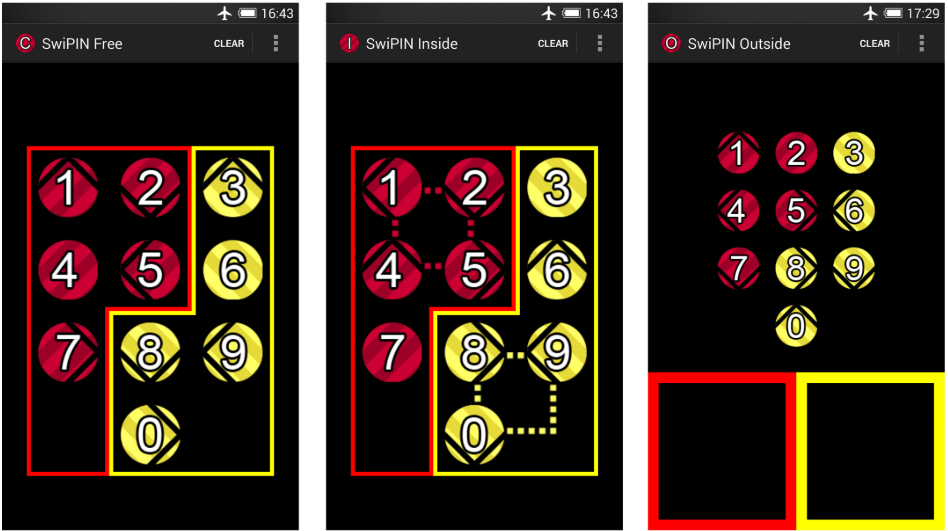
\includegraphics[width=13cm, height=7cm]{Chapters/graphics/swipin.PNG}
\caption{The three variations of \textbf{SwiPIN} by Zezschwitz et al. \cite{Swipin}. The version that was proven to be most usable is \textbf{SwiPIN} \textit{(outside}) on the far right \cite{Swipin}. }
\label{fig:swipin}
\end{figure}


\subsection{Approaches towards Novel Authentication Concepts}

In addition to the earlier discussed research and findings, researchers have also contributed to proposing novel authentication methods. Although their intentions were primarily directed towards solving certain security issues, such as smudge and shoulder surfing attacks (Section \ref{2.1.1}). They also introduced unique authentication methods that might be more usable than existing ones. Moreover, they made certain discoveries along the way that influence the approach of evaluating usability.\\

Zezschwitz et al. \cite{Swipin} created an interesting mechanism called \textbf{SwiPIN} (see figure \ref{fig:swipin}). It was intended to be support the original PIN method in situations in which stronger authentication security is needed. Its main purpose was to prevent shoulder surfing attacks when users authenticate with their pin. Zezschwitz et al \cite{Swipin} created three variations of the concept, of which one proved to have the best usability of them all, \textbf{SwiPIN} \textit{(outside)} (see figure \ref{fig:swipin}). The idea of the concept is to enter the pin through gestures rather than through tapping the buttons (numbers). The interface presents a number pad and on each of the buttons there is a black arrow which indicates the direction in which the gestures should be performed, and a specific color (yellow or red). To enter one's pin one would simply perform the gestures of the respective numbers in one of two "boxes" displayed at the bottom of the screen. Gestures of red buttons are performed in the red box and gestures of yellow buttons, in the yellow box (see figure \ref{fig:swipin}). The gesture which was assigned to each number changed for each authentication run. Remarkably, this design increased the effort and memory needed to "successfully" perform a shoulder surfing attack because the attacker must try to memorize the gestures, their order and the color of the boxes in which they are performed in order to find out which numbers were entered. \\

\begin{figure}[t!]
\centering
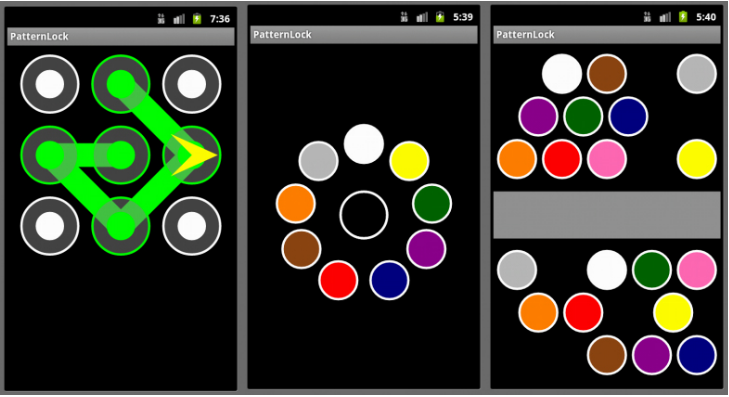
\includegraphics[width=13cm, height=7cm]{Chapters/graphics/graphic.PNG}
\caption{The three concepts made by Zezschwitz et al. \cite{Marbles}. (Left) Pattern 90, a special version of Pattern Rotation, (Middle) Marbles, (Right) Marble Gap, a variation of Marbles.}
\label{fig:marbles}
\end{figure}

Zezschwitz et al. \cite{Swipin} further conducted a study where \textbf{SwiPIN} and the original PIN where compared to each other. Although the utilization of \textbf{SwiPIN} lead to a slightly longer authentication process than PIN. A noticed disadvantage of the concept, was that users had to approach it differently than PIN. Entering a memorized pin into a number pad is based more on muscle memory and less on the digit sequence. Therefore, when using \textbf{SwiPIN}, users had to consciously recall their pin, instead of entering in "blindly". Nonetheless, all participants of the study approved of the concept and imagined themselves using it in risky situations. \\

Another contribution towards designing novel security concepts was made by Zezschwitz et al. \cite{Marbles}. Their goal was to create a protection mechanism against smudge attacks (Section \ref{2.1.1}). They created three concepts: \textbf{Marbles}, \textbf{Marble Gap} and \textbf{Pattern Rotation} (see figure \ref{fig:marbles}). The idea for \textbf{Marbles} was to create an interface which presented colored dots (marbles) aligned in a circular order. The marbles represented the elements which defined a specific password. In order to authenticate, the user would enter their password by dragging in the marbles in the center circle, in the right order. \textbf{Marble Gap} was based on the same idea, yet differed in its mapping. The marbles were displayed at the top and bottom of the display, separated by a centered rectangle (gap). To enter the password, the user had to drag in the marbles, either from the top or bottom, into the gap. It is important to note that the arrangement and display of the marbles was random for each authentication run, in both concepts. The concept of \textbf{Pattern Rotation} was based on the traditional Android Unlock Pattern mechanism. The interface presented a 3x3 grid of nodes, which changed its orientation every time a user wanted to authenticate. A special version of \textbf{Pattern Rotation}, Pattern 90, had enabled four different grid orientation (see figure \ref{fig:marbles}. \\

To examine which one of the three concepts users' preferred best in terms of usability and effectiveness, Zezschwitz et al. \cite{Marbles} conducted a study in which all three concepts were analyzed. They adopted an interesting approach, to measure the authentication times. They dissected the authentication process into "orientation" and "input" time. Interestingly, Harbach et al. \cite{AnatomySmartphone} made a similar approach through when they analyzed the difference between PIN and PATTERN (Section \ref{2.2.2}). Zezschwitz et al. \cite{Marbles} defined the "orientation" to be the the period between the beginning of the authentication and the first input event of the user. Also, they interpreted the input time as the period between the first input event and the moment in which the input is approved or cancelled. Through this distinction they realized that the factor of randomization in each of the concepts affected the overall authentication time in different parts. For instance, in \textbf{Marbles} and in \textbf{Marble Gap}, randomization was shown to elongate the "input" time, because the elements, which they needed for their input, were positioned differently every time. In contrast, the orientation time of Pattern Rotation was increased through randomization because participants needed more time to familiarize with the current position of the grid. Another discovery made, through the distinction of "orientation" and "input", was participants' perception of speed. While \textbf{Pattern Rotation} was measured to be the second quickest of all three, participants rated it as the slowest. However, \textbf{Pattern Rotation} did have the longest orientation time. This discovery allowed Zezschwitz et al. \cite{Marbles} to realize that users disliked mechanisms that had a long "orientation" time, accompanied with a long "input" time. Therefore, \textbf{Pattern Rotation} was considered not usable. Security analysis also showed it to not sufficiently seucre, also. In contrast, participants approved of \textbf{Marbles} and \textbf{Marbles Gap} and considered them very usable.\\


Looking back at the reasearch contributions discussed in this chapter, we noticed that one of the main reasons why users were found to consciously discard authentication mechanism for their smartphones was due to "inconvenience" [QUELLE]. Despite attempting to attract smartphone users to use screen locks by informing them about their effectiveness and purpose \cite{Albayram:2017:BUL:3235924.3235929}, a decent amount of study participants were found to not improve their security behavior. As mentioned earlier, smartphone users were found claimed to agree on using a screen lock, if the particular mechanism promised to be faster than the already existing ones \cite{AnatomySmartphone}. This indicated that users prefer efficiency over effectiveness. However, previously discussed findings by Zezschwitz et al. \cite{PatternWild} have shown that the efficiency of an authentication mechanism can not be determined by the time that it requires for unlocking. Although PIN proved to take less time to authenticate than PATTERN, study participants preferred the pattern mechanism better \cite{PatternWild}. Reason being that they had to prepare for authenticating with PIN longer than for the authentication with PATTERN \cite{AnatomySmartphone}. Consequently, we learned that in order to examine the efficiency of a particular authentication mechanism, we can not solely rely on comparing their measured input time. This revelation was backed by the approach of Zezschwitz et al. \cite{Marbles}. By dividing the authentication time into "orientation" and "input" time they not only understood users' perception of efficiency better but were also able to detect how differently certain design choices (e.g., randomization) can influence the anatomy of particular authentication mechanisms. \\

Thus Users' perceive interactions that require less cognitive effort to be more efficient and faster to use. We have learned that measured efficiency of authentication mechanisms can not set equivalent to their perceived efficiency \cite{anonymous}. On that note, examining the factors that affect perceived efficiency could be a productive step towards better understanding what types of mechanism designs users approve of or discard. In that way, researchers could evaluate existing and newly designed authentication mechanisms, and also compare them to each other, in the same manner. This introduces the main goal of our thesis, which is to contribute towards finding a standard through which we could generalize a evaluation method usability, with focus on perceived efficiency. In the course of this study we will base our work on the findings made in an unpublished paper by Anonymous et al. \cite{anonymous}. In their paper they grasped the notion of dissecting authentication time and proposed a novel method of rating usability according users' perceotion, rather than quantitative measurements. To provide a basic comprehension of our work throughout this thesis, we will introduce and explain their findings in Chapter \ref{ch:third}. 






